\section{Results}\label{sec:results}

\subsection{Accuracy and label cost}\label{sec:main}
Table~\ref{tab:rev-main} gives the stream-level results. The static detectors end between MCC {{main|Static-MLP|mcc:.3f}} and {{main|TFIDF-LR|mcc:.3f}}, and the label-on-alarm and fully supervised methods lie between {{main|KSWIN-Score|mcc:.3f}} and {{main|Online-TFIDF-SGD|mcc:.3f}}. SLIDE reaches {{main|SLIDE|mcc:.3f}} with {{main|SLIDE|labels:,.0f}} labels, which is {{=[main|SLIDE|labels]/[main|Online-TFIDF-SGD|labels]:.1%}} of the {{main|Online-TFIDF-SGD|labels:,.0f}} labels that the fully supervised methods consume. The online TF-IDF learner is the most accurate method ({{main|Online-TFIDF-SGD|mcc:.3f}}) and ranks first in every realisation; SLIDE is {{=-[vs|Online-TFIDF-SGD|d]:.3f}} MCC below it and loses all ten paired realisations ($p_{\mathrm{Holm}}={{vs|Online-TFIDF-SGD|ph:.4f}}$, Table~\ref{tab:rev-stats}). ADWIN-triggered retraining of the same head with all labels reaches {{main|ADWIN-Retrain|mcc:.3f}}, which SLIDE does not separate from ({{vs|ADWIN-Retrain|wins:.0f}} wins out of ten, $p_{\mathrm{Holm}}={{vs|ADWIN-Retrain|ph:.2f}}$).

\begin{table*}[t]
\centering
\caption{Prequential results on the seven-segment stream A--G (36{,}000 messages, mean\,$\pm$\,95\% CI half-width over 10 realisations). Labels: stream labels consumed after warm-up; Upd.: model updates per stream. The Budget-* rows spend the same number of labels as SLIDE, either spread over the stream (uniform, uncertainty) or as four windows at random batches or right after each true change (oracle).}
\label{tab:rev-main}
\scriptsize
\setlength{\tabcolsep}{3pt}
\resizebox{\textwidth}{!}{\begin{tabular}{@{}lccccccc@{}}
\toprule
Method & Precision & Recall & MCC & PR-AUC & FPR & Labels & Upd. \\
\midrule
TFIDF-LR & 0.759\,$\pm$\,0.001 & 0.891\,$\pm$\,0.001 & 0.702\,$\pm$\,0.001 & 0.877\,$\pm$\,0.001 & 0.172\,$\pm$\,0.001 & 0 & 0.0 \\
Online-TFIDF-SGD & 0.941\,$\pm$\,0.003 & 0.939\,$\pm$\,0.001 & 0.904\,$\pm$\,0.002 & 0.980\,$\pm$\,0.001 & 0.036\,$\pm$\,0.002 & 35500 & every batch \\
Static-FT & 0.881\,$\pm$\,0.001 & 0.688\,$\pm$\,0.002 & 0.671\,$\pm$\,0.001 & 0.901\,$\pm$\,0.001 & 0.056\,$\pm$\,0.000 & 0 & 0.0 \\
\midrule
Static-MLP & 0.846\,$\pm$\,0.002 & 0.719\,$\pm$\,0.004 & 0.664\,$\pm$\,0.002 & 0.855\,$\pm$\,0.003 & 0.079\,$\pm$\,0.001 & 0 & 0.0 \\
Online-MLP & 0.915\,$\pm$\,0.003 & 0.940\,$\pm$\,0.001 & 0.883\,$\pm$\,0.003 & 0.972\,$\pm$\,0.001 & 0.053\,$\pm$\,0.002 & 35500 & every batch \\
ADWIN-Retrain & 0.927\,$\pm$\,0.004 & 0.937\,$\pm$\,0.003 & 0.891\,$\pm$\,0.003 & 0.973\,$\pm$\,0.002 & 0.045\,$\pm$\,0.003 & 35500 & 5.6 \\
KSWIN-Score & 0.926\,$\pm$\,0.004 & 0.907\,$\pm$\,0.013 & 0.867\,$\pm$\,0.012 & 0.966\,$\pm$\,0.006 & 0.044\,$\pm$\,0.002 & 9700 & 19.4 \\
Budget-Uniform-MLP & 0.871\,$\pm$\,0.005 & 0.905\,$\pm$\,0.002 & 0.818\,$\pm$\,0.005 & 0.944\,$\pm$\,0.003 & 0.082\,$\pm$\,0.004 & 2982 & 0.0 \\
\midrule
Budget-Uncertainty-MLP & 0.921\,$\pm$\,0.007 & 0.815\,$\pm$\,0.013 & 0.794\,$\pm$\,0.008 & 0.926\,$\pm$\,0.005 & 0.043\,$\pm$\,0.005 & 2982 & 0.0 \\
Budget-Uniform-TFIDF & 0.890\,$\pm$\,0.006 & 0.898\,$\pm$\,0.007 & 0.829\,$\pm$\,0.007 & 0.954\,$\pm$\,0.003 & 0.067\,$\pm$\,0.004 & 2982 & 0.0 \\
Budget-Uncertainty-TFIDF & 0.917\,$\pm$\,0.006 & 0.873\,$\pm$\,0.008 & 0.834\,$\pm$\,0.006 & 0.955\,$\pm$\,0.004 & 0.048\,$\pm$\,0.004 & 2982 & 0.0 \\
Budget-Random & 0.867\,$\pm$\,0.024 & 0.851\,$\pm$\,0.027 & 0.774\,$\pm$\,0.033 & 0.917\,$\pm$\,0.019 & 0.080\,$\pm$\,0.016 & 3000 & 5.5 \\
Budget-Oracle & 0.929\,$\pm$\,0.003 & 0.936\,$\pm$\,0.002 & 0.891\,$\pm$\,0.002 & 0.969\,$\pm$\,0.002 & 0.044\,$\pm$\,0.002 & 3000 & 6.0 \\
Budget-Random-TFIDF & 0.843\,$\pm$\,0.027 & 0.856\,$\pm$\,0.042 & 0.756\,$\pm$\,0.038 & 0.920\,$\pm$\,0.020 & 0.098\,$\pm$\,0.020 & 3000 & 5.5 \\
Budget-Oracle-TFIDF & 0.930\,$\pm$\,0.004 & 0.929\,$\pm$\,0.002 & 0.887\,$\pm$\,0.004 & 0.976\,$\pm$\,0.002 & 0.042\,$\pm$\,0.002 & 3000 & 6.0 \\
\midrule
SLIDE (earlier design) & 0.924\,$\pm$\,0.004 & 0.937\,$\pm$\,0.002 & 0.888\,$\pm$\,0.003 & 0.967\,$\pm$\,0.002 & 0.047\,$\pm$\,0.003 & 3000 & 6.0 \\
\textbf{SLIDE} & 0.927\,$\pm$\,0.004 & 0.936\,$\pm$\,0.004 & 0.889\,$\pm$\,0.003 & 0.969\,$\pm$\,0.002 & 0.045\,$\pm$\,0.003 & 3000 & 6.0 \\
\textbf{SLIDE}+replay & 0.921\,$\pm$\,0.004 & 0.936\,$\pm$\,0.003 & 0.884\,$\pm$\,0.003 & 0.964\,$\pm$\,0.002 & 0.049\,$\pm$\,0.003 & 3000 & 6.0 \\
\textbf{SLIDE}-TFIDF & 0.924\,$\pm$\,0.005 & 0.933\,$\pm$\,0.004 & 0.885\,$\pm$\,0.004 & 0.975\,$\pm$\,0.001 & 0.047\,$\pm$\,0.003 & 3000 & 6.0 \\
\bottomrule
\end{tabular}}
\end{table*}


The earlier design with the four-term objective and surprisal features reaches {{main|SLIDE (KBS version)|mcc:.3f}}, statistically indistinguishable from the revised SLIDE ($p_{\mathrm{Holm}}={{vs|SLIDE (KBS version)|ph:.2f}}$) at {{=[main|SLIDE (KBS version)|t_update]/[main|SLIDE|t_update]:.1f}} times the update time. KSWIN on the score spends {{main|KSWIN-Score|labels:,.0f}} labels in {{main|KSWIN-Score|updates:.1f}} purchases and ends {{vs|KSWIN-Score|d:.3f}} MCC below SLIDE ({{vs|KSWIN-Score|wins:.0f}}/10, $p_{\mathrm{Holm}}={{vs|KSWIN-Score|ph:.4f}}$). The Friedman test rejects equal performance across the {{n_methods:.0f}} methods ($\chi^2_F={{friedman_chi2:.1f}}$); with a Nemenyi critical difference of {{nemenyi_cd:.2f}} ranks, SLIDE (mean rank {{rank|SLIDE:.1f}}) is separated from the static detectors and from the uniform, uncertainty and random-time samplers with the head, but not from the other adaptive methods.

\begin{table}[t]
\centering
\caption{Revised SLIDE against each method on the A--G stream: mean paired MCC difference, wins out of 10 realisations, two-sided Wilcoxon signed-rank test with Holm correction over 18 comparisons, rank-biserial effect size $r_{rb}$, and Friedman mean rank (Friedman $\chi^2_F=166.7$, $p=4.1e-26$; Nemenyi CD$_{0.05}=8.85$).}
\label{tab:rev-stats}
\scriptsize
\setlength{\tabcolsep}{3pt}
\begin{tabular}{@{}lccccc@{}}
\toprule
Competitor & $\Delta$MCC & wins & $p_{\mathrm{Holm}}$ & $r_{rb}$ & rank \\
\midrule
TFIDF-LR & +0.187 & 10/10 & 0.0352 & +1.00 & 16.7 \\
Online-TFIDF-SGD & -0.015 & 0/10 & 0.0352 & -1.00 & 1.0 \\
Static-FT & +0.218 & 10/10 & 0.0352 & +1.00 & 17.9 \\
Static-MLP & +0.225 & 10/10 & 0.0352 & +1.00 & 19.0 \\
Online-MLP & +0.006 & 8/10 & 0.117 & +0.82 & 7.5 \\
ADWIN-Retrain & -0.002 & 3/10 & 0.48 & -0.53 & 3.9 \\
KSWIN-Score & +0.022 & 9/10 & 0.0352 & +0.96 & 8.9 \\
Budget-Uniform-MLP & +0.071 & 10/10 & 0.0352 & +1.00 & 13.2 \\
Budget-Uncertainty-MLP & +0.095 & 10/10 & 0.0352 & +1.00 & 14.8 \\
Budget-Uniform-TFIDF & +0.060 & 10/10 & 0.0352 & +1.00 & 11.9 \\
Budget-Uncertainty-TFIDF & +0.055 & 10/10 & 0.0352 & +1.00 & 11.4 \\
Budget-Random & +0.115 & 10/10 & 0.0352 & +1.00 & 14.5 \\
Budget-Oracle & -0.002 & 3/10 & 0.322 & -0.67 & 3.8 \\
Budget-Random-TFIDF & +0.133 & 10/10 & 0.0352 & +1.00 & 15.6 \\
Budget-Oracle-TFIDF & +0.002 & 6/10 & 0.48 & +0.31 & 5.6 \\
SLIDE (earlier design) & +0.001 & 8/10 & 0.422 & +0.60 & 5.6 \\
SLIDE+replay & +0.005 & 9/10 & 0.041 & +0.93 & 7.5 \\
SLIDE-TFIDF & +0.004 & 6/10 & 0.48 & +0.49 & 6.4 \\
\midrule
SLIDE (mean rank) &  &  &  &  & 4.8 \\
\bottomrule
\end{tabular}
\end{table}


Table~\ref{tab:rev-segments} locates the differences. On the human segments A--C, SLIDE is within 0.02 MCC of the best method in each. The gap to the online TF-IDF learner is concentrated in the LLM segment D ({{main|SLIDE|mcc|D:.3f}} against {{main|Online-TFIDF-SGD|mcc|D:.3f}}) and in the PhishFuzzer segment F ({{main|SLIDE|mcc|F:.3f}} against {{main|Online-TFIDF-SGD|mcc|F:.3f}}). In both, the TF-IDF learner receives every label from the first batch of the segment on, while SLIDE scores with the previous head until its purchased window arrives. SLIDE-TFIDF, which buys the same labels at the same alarms but updates the TF-IDF learner, closes most of the segment-F gap ({{main|SLIDE-TFIDF|mcc|F:.3f}}) and a third of the segment-D gap ({{main|SLIDE-TFIDF|mcc|D:.3f}}). Figure~\ref{fig:rev-trajectory} shows the batch-level picture: the head-based methods dip at the first batches of D and F and recover once labels arrive, and the static head stays near MCC 0.2--0.4 on the LLM segments.

\begin{table*}[t]
\centering
\caption{MCC per segment of the A--G stream (mean over 10 realisations; best per column in bold).}
\label{tab:rev-segments}
\scriptsize
\setlength{\tabcolsep}{3pt}
\resizebox{\textwidth}{!}{\begin{tabular}{@{}lccccccc@{}}
\toprule
Method & A & B & C & D & E & F & G \\
\midrule
TFIDF-LR & \textbf{0.956} & 0.825 & 0.891 & 0.433 & 0.570 & 0.708 & 0.405 \\
Online-TFIDF-SGD & 0.925 & 0.869 & 0.920 & \textbf{0.892} & \textbf{0.899} & \textbf{0.895} & \textbf{0.889} \\
Static-FT & 0.948 & 0.824 & 0.711 & 0.221 & 0.433 & 0.453 & 0.665 \\
Static-MLP & 0.951 & 0.832 & 0.719 & 0.236 & 0.443 & 0.375 & 0.659 \\
Online-MLP & 0.945 & 0.889 & \textbf{0.922} & 0.769 & 0.898 & 0.843 & 0.841 \\
ADWIN-Retrain & 0.951 & \textbf{0.892} & 0.915 & 0.827 & 0.864 & 0.833 & 0.870 \\
KSWIN-Score & 0.947 & 0.877 & 0.896 & 0.757 & 0.843 & 0.820 & 0.828 \\
Budget-Uniform-MLP & 0.949 & 0.854 & 0.875 & 0.618 & 0.807 & 0.759 & 0.731 \\
Budget-Uncertainty-MLP & 0.946 & 0.871 & 0.787 & 0.471 & 0.817 & 0.813 & 0.759 \\
Budget-Uniform-TFIDF & 0.922 & 0.793 & 0.859 & 0.758 & 0.815 & 0.809 & 0.754 \\
Budget-Uncertainty-TFIDF & 0.916 & 0.823 & 0.806 & 0.752 & 0.861 & 0.868 & 0.774 \\
Budget-Random & 0.949 & 0.864 & 0.768 & 0.548 & 0.810 & 0.766 & 0.624 \\
Budget-Oracle & 0.951 & \textbf{0.893} & 0.915 & 0.815 & 0.883 & 0.844 & 0.856 \\
Budget-Random-TFIDF & 0.941 & 0.834 & 0.745 & 0.573 & 0.782 & 0.808 & 0.569 \\
Budget-Oracle-TFIDF & 0.941 & 0.858 & 0.897 & 0.852 & 0.872 & 0.894 & 0.848 \\
SLIDE (earlier design) & 0.950 & 0.879 & 0.915 & 0.825 & 0.896 & 0.835 & 0.839 \\
SLIDE & 0.951 & 0.880 & 0.915 & 0.818 & 0.885 & 0.842 & 0.860 \\
SLIDE+replay & 0.951 & 0.878 & 0.913 & 0.820 & 0.887 & 0.826 & 0.834 \\
SLIDE-TFIDF & 0.941 & 0.849 & 0.895 & 0.841 & 0.871 & 0.892 & 0.859 \\
\bottomrule
\end{tabular}}
\end{table*}


\begin{figure*}[t]
\centering
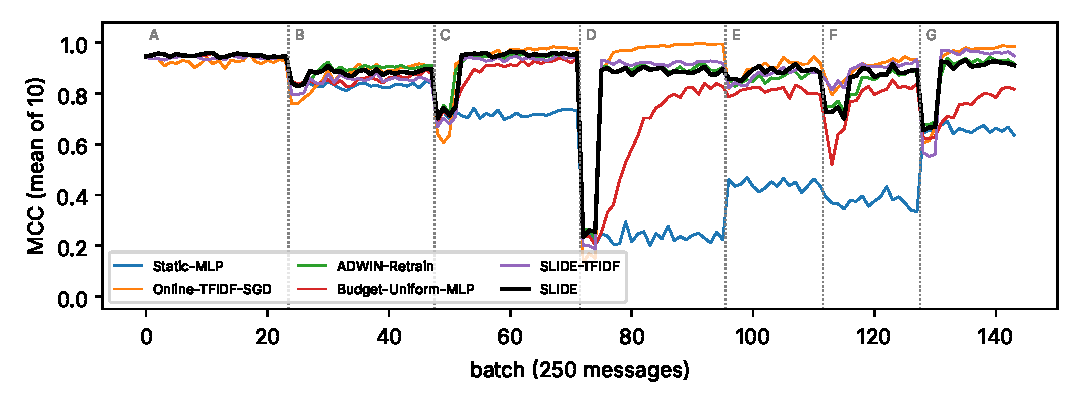
\includegraphics[width=\textwidth]{figures/rev_trajectory.pdf}
\caption{Batch MCC along the A--G stream (mean over 10 realisations). Dotted lines mark segment boundaries.}
\label{fig:rev-trajectory}
\end{figure*}

\subsection{When to buy labels: equal-budget controls}\label{sec:budgetctrl}
The equal-budget rows of Table~\ref{tab:rev-main} hold the learner and the number of labels fixed and vary only when the labels are bought. With the head, spreading {{main|SLIDE|labels:,.0f}} labels uniformly over the stream gives {{main|Budget-Uniform-MLP|mcc:.3f}}, choosing the most uncertain messages gives {{main|Budget-Uncertainty-MLP|mcc:.3f}} and buying six windows at random batches gives {{main|Budget-Random|mcc:.3f}}. SLIDE exceeds each of them in all ten realisations by {{vs|Budget-Uniform-MLP|d:.3f}}, {{vs|Budget-Uncertainty-MLP|d:.3f}} and {{vs|Budget-Random|d:.3f}} MCC ($p_{\mathrm{Holm}}={{p_min_holm:.4f}}$ each, the smallest value the design allows). An oracle that buys a window as soon as 500 messages of each new segment exist reaches {{main|Budget-Oracle|mcc:.3f}}, {{=-[vs|Budget-Oracle|d]:.3f}} above SLIDE and not significantly so ($p_{\mathrm{Holm}}={{vs|Budget-Oracle|ph:.2f}}$). The same ordering holds with the TF-IDF learner: uniform {{main|Budget-Uniform-TFIDF|mcc:.3f}}, uncertainty {{main|Budget-Uncertainty-TFIDF|mcc:.3f}}, random times {{main|Budget-Random-TFIDF|mcc:.3f}}, SLIDE-TFIDF {{main|SLIDE-TFIDF|mcc:.3f}} and oracle {{main|Budget-Oracle-TFIDF|mcc:.3f}}. The trigger thus captures almost all of the value that knowledge of the true boundaries would give, for either learner, and the samplers that ignore the shift lose 0.05--0.13 MCC at the same cost.

The uniform sampler loses most on the LLM segment D ({{main|Budget-Uniform-MLP|mcc|D:.3f}} against {{main|SLIDE|mcc|D:.3f}} for SLIDE). Twenty-one labels per batch arrive throughout D, but three epochs on each small set evidently do not move the head as far from the human-mail regime as one update on 500 labels of the new segment. Uncertainty sampling is worse than uniform sampling with the head ({{main|Budget-Uncertainty-MLP|mcc|D:.3f}} on D). This is consistent with a head that is confidently wrong on the new LLM traffic, so that the messages near a score of 0.5 are not the ones it misclassifies.

\subsection{Ablation and retention}\label{sec:ablation}
Table~\ref{tab:rev-ablation} removes or replaces one component at a time. Adaptation is necessary: without it the detector stays at the static level ({{abl|revised, no adaptation|mcc:.3f}}). The projections carry the trigger: a test on the score alone raises fewer alarms, buys {{abl|revised, score-only test|labels:,.0f}} labels and ends at {{abl|revised, score-only test|mcc:.3f}} ($p_{\mathrm{Holm}}={{abl|revised, score-only test|p:.4f}}$), while the projections-only test reproduces SLIDE. Either gate alone raises the same alarms on this stream; on stationary traffic the SW gate alone does not (Section~\ref{sec:null}). None of the update variants changes stream MCC measurably: the full four-term objective with or without $\psi$, warm start with replay, warm start without replay and retraining from scratch all lie within {{=abs([abl|warm+replay|d]):.3f}} MCC of the revised configuration ($p_{\mathrm{Holm}}\geq{{abl|warm+replay|p:.3f}}$). The surprisal features $\psi$ add nothing ({{abl|warm + psi|mcc:.3f}} with, {{abl|warm (revised update)|mcc:.3f}} without).

\begin{table*}[t]
\centering
\caption{Component ablation on the A--G stream (10 realisations). $\Delta$ and $p_{\mathrm{Holm}}$ compare each variant with the revised configuration (warm-start update, no $\psi$, $\alpha$-spending) by a two-sided Wilcoxon test on realisation-level MCC, Holm-corrected. Upd.\,s: total update time per stream in seconds.}
\label{tab:rev-ablation}
\scriptsize
\setlength{\tabcolsep}{3pt}
\resizebox{\textwidth}{!}{\begin{tabular}{@{}lcccccccc@{}}
\toprule
Variant & MCC & PR-AUC & MCC (F) & MCC (G) & Labels & Upd.\,s & $\Delta$ & $p_{\mathrm{Holm}}$ \\
\midrule
full objective + $\psi$ (earlier design) & 0.888\,$\pm$\,0.003 & 0.967 & 0.835 & 0.839 & 3000 & 914.4 & -0.001 & 0.844 \\
full objective, no $\psi$ & 0.887\,$\pm$\,0.003 & 0.966 & 0.834 & 0.839 & 3000 & 867.4 & -0.002 & 1 \\
warm+replay & 0.884\,$\pm$\,0.003 & 0.963 & 0.827 & 0.829 & 3000 & 253.1 & -0.005 & 0.0527 \\
warm (revised update) & 0.889\,$\pm$\,0.002 & 0.969 & 0.844 & 0.857 & 3000 & 150.0 & +0.000 & 1 \\
scratch & 0.890\,$\pm$\,0.003 & 0.974 & 0.844 & 0.874 & 3000 & 144.0 & +0.001 & 1 \\
warm + $\psi$ & 0.890\,$\pm$\,0.002 & 0.969 & 0.845 & 0.855 & 3000 & 147.7 & +0.001 & 1 \\
revised + $\alpha$-spending & 0.889\,$\pm$\,0.003 & 0.969 & 0.842 & 0.860 & 3000 & 138.1 & -- & -- \\
revised, KS gate only & 0.889\,$\pm$\,0.002 & 0.969 & 0.842 & 0.860 & 3000 & 140.1 & +0.000 & 1 \\
revised, SW gate only & 0.889\,$\pm$\,0.002 & 0.969 & 0.843 & 0.857 & 3000 & 142.7 & +0.000 & 1 \\
revised, score-only test & 0.828\,$\pm$\,0.010 & 0.936 & 0.742 & 0.846 & 1300 & 62.1 & -0.061 & 0.0215 \\
revised, projections-only & 0.889\,$\pm$\,0.003 & 0.969 & 0.842 & 0.860 & 3000 & 150.0 & +0.000 & 1 \\
revised, no adaptation & 0.664\,$\pm$\,0.002 & 0.855 & 0.375 & 0.659 & 0 & 0.0 & -0.225 & 0.0215 \\
\bottomrule
\end{tabular}}
\end{table*}


Prequential MCC measures accuracy on the traffic at hand, not what a detector keeps from earlier campaigns. Table~\ref{tab:rev-retention} measures retention directly on a held-out pool from the sources of segments B--D. Every learner that updates only on recent data forgets: just before segment E SLIDE detects {{ret|SLIDE|preE:.3f}} of the pool, at the end of the stream {{ret|SLIDE|end:.3f}}; ADWIN-Retrain falls from {{ret|ADWIN-Retrain|preE:.3f}} to {{ret|ADWIN-Retrain|end:.3f}} and the oracle schedule from {{ret|Budget-Oracle|preE:.3f}} to {{ret|Budget-Oracle|end:.3f}}. Class-balanced replay removes the loss. With replay SLIDE keeps {{ret|SLIDE+replay|end:.3f}} at the end, the earlier design keeps {{ret|SLIDE (KBS version)|end:.3f}}, and the online TF-IDF learner, which never discards its weights, keeps {{ret|Online-TFIDF-SGD|end:.3f}}. Stream MCC cannot show this effect, because the stream never returns to an earlier source. Retention has a price on the current traffic. SLIDE+replay reaches stream MCC {{main|SLIDE+replay|mcc:.3f}} (Table~\ref{tab:rev-main}), {{vs|SLIDE+replay|d:.3f}} below SLIDE in {{vs|SLIDE+replay|wins:.0f}} of ten realisations ($p_{\mathrm{Holm}}={{vs|SLIDE+replay|ph:.3f}}$), at {{=[main|SLIDE+replay|t_update]/[main|SLIDE|t_update]:.1f}} times the update time, because part of every update is spent on earlier sources. The choice between the two is an operating decision: SLIDE when only the current traffic matters, SLIDE+replay when old campaigns may return.

\begin{table}[t]
\centering
\caption{Retention: detection rate on 600 held-out malicious messages from the sources of segments B--D (400 GPTGen and SpearGen, 200 TREC and CEAS-08), never streamed, scored by each detector as it stands before the stream ($t_0$), just before segment E and at the end of the stream (mean over 10 realisations). $\Delta$: end minus pre-E.}
\label{tab:rev-retention}
\scriptsize
\setlength{\tabcolsep}{3pt}
\begin{tabular}{@{}lcccc@{}}
\toprule
Method & $t_0$ & pre-E & end & $\Delta$ \\
\midrule
TFIDF-LR & 0.712 & 0.712 & 0.712 & +0.000 \\
Online-TFIDF-SGD & 0.703 & 0.797 & 0.794 & -0.003 \\
Static-FT & 0.417 & 0.417 & 0.417 & +0.000 \\
\midrule
Static-MLP & 0.458 & 0.458 & 0.458 & +0.000 \\
Online-MLP & 0.458 & 0.904 & 0.842 & -0.062 \\
ADWIN-Retrain & 0.458 & 0.938 & 0.530 & -0.407 \\
KSWIN-Score & 0.458 & 0.728 & 0.425 & -0.302 \\
Budget-Uniform-MLP & 0.458 & 0.864 & 0.660 & -0.204 \\
\midrule
Budget-Uncertainty-MLP & 0.458 & 0.682 & 0.637 & -0.045 \\
Budget-Uniform-TFIDF & 0.703 & 0.860 & 0.761 & -0.100 \\
Budget-Uncertainty-TFIDF & 0.703 & 0.790 & 0.771 & -0.019 \\
Budget-Random & 0.458 & 0.786 & 0.750 & -0.036 \\
Budget-Oracle & 0.458 & 0.907 & 0.651 & -0.256 \\
Budget-Random-TFIDF & 0.703 & 0.770 & 0.768 & -0.002 \\
Budget-Oracle-TFIDF & 0.703 & 0.851 & 0.738 & -0.113 \\
\midrule
SLIDE (earlier design) & 0.459 & 0.948 & 0.948 & -0.000 \\
SLIDE & 0.458 & 0.937 & 0.659 & -0.279 \\
SLIDE+replay & 0.458 & 0.947 & 0.941 & -0.005 \\
SLIDE-TFIDF & 0.703 & 0.917 & 0.771 & -0.145 \\
\bottomrule
\end{tabular}
\end{table}


\subsection{Number of projections and label window}\label{sec:K}
Table~\ref{tab:rev-K} varies the number of random projections. With $K=2$ the test misses {{K|2|miss:.0%}} of the boundaries and SLIDE ends at MCC {{K|2|mcc:.3f}}; from $K=8$ on it misses at most one boundary in 30, and from $K=64$ on none. Stream MCC is flat between $K=32$ ({{K|32|mcc:.3f}}) and $K=512$ ({{K|512|mcc:.3f}}), and the mean detection delay stays between {{K|512|delay:.1f}} and {{K|128|delay:.1f}} batches over that range. The test time per stream grows from {{K|2|t_detect:.0f}}\,s at $K=2$ to {{K|64|t_detect:.0f}}\,s at the default $K=64$ and {{K|512|t_detect:.0f}}\,s at $K=512$. No setting raised an alarm inside a segment. The share of individually significant projections falls from {{K|2|frac_sig:.2f}} to {{K|512|frac_sig:.2f}} as $K$ grows, so a shift moves a minority of directions and more projections mainly add directions that the shift does not touch; $K=64$ is the smallest value without misses.

\begin{table}[t]
\centering
\caption{Number of random projections $K$ (revised SLIDE, 5 realisations, six boundaries per stream). Delay: batches from a boundary to the first alarm in the new segment; miss: share of boundaries without an alarm before the next boundary; extra: further alarms per stream; sig.: share of projections individually significant at the Holm level in alarming tests; CV$_{W_1}$: coefficient of variation of the per-projection $W_1$ distances; $t$: total test time (s).}
\label{tab:rev-K}
\scriptsize
\setlength{\tabcolsep}{3pt}
\begin{tabular}{@{}lccccccccc@{}}
\toprule
$K$ & MCC & Labels & Alarms & Delay & Miss & Extra & Sig. & CV$_{W_1}$ & $t$ \\
\midrule
2 & 0.868\,$\pm$\,0.019 & 2300 & 4.6 & 1.83 & 0.23 & 0.0 & 0.43 & 0.21 & 14.1 \\
4 & 0.875\,$\pm$\,0.024 & 2500 & 5.0 & 1.00 & 0.17 & 0.0 & 0.35 & 0.35 & 14.3 \\
8 & 0.885\,$\pm$\,0.008 & 2900 & 5.8 & 1.31 & 0.03 & 0.0 & 0.32 & 0.36 & 14.6 \\
16 & 0.885\,$\pm$\,0.010 & 2900 & 5.8 & 0.93 & 0.03 & 0.0 & 0.24 & 0.38 & 17.0 \\
32 & 0.887\,$\pm$\,0.003 & 2900 & 5.8 & 0.59 & 0.03 & 0.0 & 0.23 & 0.38 & 23.0 \\
64 & 0.888\,$\pm$\,0.002 & 3000 & 6.0 & 0.53 & 0.00 & 0.0 & 0.20 & 0.40 & 32.1 \\
128 & 0.887\,$\pm$\,0.003 & 3000 & 6.0 & 0.73 & 0.00 & 0.0 & 0.20 & 0.39 & 52.1 \\
256 & 0.888\,$\pm$\,0.003 & 3000 & 6.0 & 0.70 & 0.00 & 0.0 & 0.20 & 0.40 & 77.7 \\
512 & 0.887\,$\pm$\,0.003 & 3000 & 6.0 & 0.50 & 0.00 & 0.0 & 0.17 & 0.39 & 125.9 \\
\bottomrule
\end{tabular}
\end{table}


Table~\ref{tab:rev-budget} varies the label window $n_\ell$ bought at each alarm. Below one batch ($n_\ell<250$) the window is a random subset of the alarm batch. With $n_\ell=50$ SLIDE spends {{budget|SLIDE|50|labels:,.0f}} labels and reaches {{budget|SLIDE|50|mcc:.3f}}; with $n_\ell=100$, {{budget|SLIDE|100|labels:,.0f}} labels and {{budget|SLIDE|100|mcc:.3f}}; with one batch, {{budget|SLIDE|250|mcc:.3f}}. Fifty labels per alarm, {{budget|SLIDE|50|labels:,.0f}} in all, already match uniform sampling with {{main|Budget-Uniform-MLP|labels:,.0f}} labels ({{main|Budget-Uniform-MLP|mcc:.3f}}, Table~\ref{tab:rev-main}). Doubling the default window to 1{,}000 labels per alarm adds {{=[budget|SLIDE|1000|mcc]-[budget|SLIDE|500|mcc]:.3f}} MCC for {{=[budget|SLIDE|1000|labels]-[budget|SLIDE|500|labels]:,.0f}} more labels. The TF-IDF learner needs fewer labels per alarm: SLIDE-TFIDF reaches {{budget|SLIDE-TFIDF|250|mcc:.3f}} with one batch per alarm and gains {{=[budget|SLIDE-TFIDF|500|mcc]-[budget|SLIDE-TFIDF|250|mcc]:.3f}} from doubling it.

\begin{table}[t]
\centering
\caption{Label window $n_\ell$ bought per alarm (5 realisations). SLIDE updates the transformer head; SLIDE-TFIDF uses the same alarms to update an online TF-IDF learner.}
\label{tab:rev-budget}
\scriptsize
\setlength{\tabcolsep}{3pt}
\begin{tabular}{@{}lcccccc@{}}
\toprule
$n_\ell$ & SLIDE MCC & MCC (G) & Labels & SLIDE-TFIDF MCC & MCC (G) & Labels \\
\midrule
50 & -- & -- & -- & -- & -- & -- \\
100 & -- & -- & -- & -- & -- & -- \\
250 & -- & -- & -- & -- & -- & -- \\
500 & -- & -- & -- & -- & -- & -- \\
1000 & -- & -- & -- & -- & -- & -- \\
\bottomrule
\end{tabular}
\end{table}


\subsection{Label delay}\label{sec:delay}
Every method that learns from labels loses accuracy as labels arrive later (Table~\ref{tab:rev-delay}), because the head scores each new segment with the old model until the purchased window is delivered. SLIDE falls from {{delay|SLIDE|1:.3f}} at $D=1$ to {{delay|SLIDE|8:.3f}} at $D=8$ and {{delay|SLIDE|16:.3f}} at $D=16$. The fully supervised online TF-IDF learner falls at the same rate, from {{delay|Online-TFIDF-SGD|1:.3f}} to {{delay|Online-TFIDF-SGD|8:.3f}} and {{delay|Online-TFIDF-SGD|16:.3f}}, so its advantage over SLIDE disappears once labels are eight or more batches (2{,}000 messages) late. With random delays the gap remains: {{delay|SLIDE|rand1-16:.3f}} for SLIDE against {{delay|Online-TFIDF-SGD|rand1-16:.3f}} for the online learner when delays range over 1--16 batches, because the online learner uses each early label as soon as it arrives, while SLIDE waits for the whole window. The uniform equal-budget sampler stays below SLIDE at every delay ({{delay|Budget-Uniform-TFIDF|1:.3f}} at $D=1$, {{delay|Budget-Uniform-TFIDF|16:.3f}} at $D=16$).

\begin{table}[t]
\centering
\caption{MCC under label delay (5 realisations, $r=0,\dots,4$). $D$ is the delay in batches of 250 messages; rand$a$--$b$ draws each batch's delay uniformly from $\{a,\dots,b\}$. $D=2$ is the default of Table~\ref{tab:rev-main}.}
\label{tab:rev-delay}
\scriptsize
\setlength{\tabcolsep}{3pt}
\begin{tabular}{@{}lccccccc@{}}
\toprule
Method & $D$=1 & $D$=2 & $D$=4 & $D$=8 & $D$=16 & rand 1-8 & rand 1-16 \\
\midrule
SLIDE & 0.898 & 0.888 & 0.870 & 0.831 & 0.745 & 0.873 & 0.819 \\
SLIDE-TFIDF & 0.896 & 0.885 & 0.863 & 0.821 & 0.740 & 0.865 & 0.808 \\
Online-TFIDF-SGD & 0.913 & 0.902 & 0.876 & 0.828 & 0.739 & 0.885 & 0.862 \\
Budget-Uniform-TFIDF & 0.837 & 0.825 & 0.804 & 0.760 & 0.692 & 0.811 & 0.785 \\
\bottomrule
\end{tabular}
\end{table}


\subsection{Stream designs}\label{sec:designs}
The ordering of Table~\ref{tab:rev-main} does not drive the result (Table~\ref{tab:rev-designs}). SLIDE ends at {{design|SLIDE|gradual:.3f}} on gradual boundaries, {{design|SLIDE|varlen:.3f}} with variable segment lengths and {{design|SLIDE|permuted:.3f}} with permuted segments, against {{design|SLIDE|abrupt:.3f}} on the default stream. On gradual boundaries it buys {{design|SLIDE|gradual|labels:,.0f}} labels instead of {{design|SLIDE|abrupt|labels:,.0f}}, because some mixing zones raise a second alarm. It also ends above the oracle schedule ({{design|Budget-Oracle|gradual:.3f}}), probably because the oracle buys its window as soon as 500 messages of the new segment exist, when the new segment is still a minority of the traffic in the mixing zone. Under every design the equal-budget samplers stay below SLIDE: uniform sampling with the head by 0.07--0.08 MCC and buying windows at random times by 0.08--0.13. The online TF-IDF learner with all labels remains the most accurate method under every design ({{design|Online-TFIDF-SGD|varlen:.3f}}--{{design|Online-TFIDF-SGD|gradual:.3f}}).

\begin{table*}[t]
\centering
\caption{MCC and labels under four stream designs (5 realisations each, $r=0,\dots,4$): abrupt (default), gradual (2{,}000-message mixing zones), variable segment lengths, and permuted segment order.}
\label{tab:rev-designs}
\scriptsize
\setlength{\tabcolsep}{3pt}
\resizebox{\textwidth}{!}{\begin{tabular}{@{}lcccccccc@{}}
\toprule
Method & abrupt MCC & Lab. & gradual MCC & Lab. & varlen MCC & Lab. & permuted MCC & Lab. \\
\midrule
SLIDE & 0.888 & 3000 & 0.886 & 3600 & 0.873 & 3000 & 0.875 & 3000 \\
SLIDE-TFIDF & 0.885 & 3000 & 0.882 & 3600 & 0.871 & 3000 & 0.873 & 3000 \\
ADWIN-Retrain & 0.889 & 35500 & 0.881 & 35500 & 0.866 & 25850 & 0.872 & 35500 \\
Online-TFIDF-SGD & 0.902 & 35500 & 0.919 & 35500 & 0.887 & 25850 & 0.899 & 35500 \\
Budget-Uniform-TFIDF & 0.825 & 2982 & 0.838 & 2982 & 0.810 & 2171 & 0.819 & 2982 \\
Budget-Uniform-MLP & 0.815 & 2982 & 0.820 & 2982 & 0.792 & 2171 & 0.809 & 2982 \\
Budget-Random & 0.782 & 3000 & 0.807 & 3000 & 0.748 & 3000 & 0.757 & 3000 \\
Budget-Oracle & 0.890 & 3000 & 0.864 & 3000 & 0.873 & 3000 & 0.871 & 3000 \\
Static-MLP & 0.664 & 0 & 0.664 & 0 & 0.651 & 0 & 0.664 & 0 \\
\bottomrule
\end{tabular}}
\end{table*}


\subsection{False alarms on a stationary stream}\label{sec:null}
On the null stream every alarm is false and every purchased window is wasted (Table~\ref{tab:rev-null}). Each realisation runs about {{null|alpha-spending|tests:.0f}} drift tests. With the per-test level $\alpha$ of the earlier design, {{null|per-test alpha|p_any:.0%}} of the streams raise at least one false alarm, and with the KS gate alone {{null|per-test alpha, KS only|p_any:.0%}}, at a cost of {{null|per-test alpha, KS only|labels:,.0f}} labels per stream on average. With harmonic $\alpha$-spending no realisation raises a false alarm, with the two gates or with the KS gate alone. The SW gate on its own, with spending, still raises a false alarm in {{null|SW gate only|p_any:.0%}} of the streams, which is the reason to keep both gates: on the A--G stream either gate alone raises the same alarms (Section~\ref{sec:ablation}), and on stationary traffic only the conjunction, or the KS gate, stays silent. KSWIN on the detector score raises {{null|KSWIN-Score|alarms:.1f}} false alarms per stream and buys {{null|KSWIN-Score|labels:,.0f}} labels for nothing. Twenty realisations bound the stream-level false-alarm rate of SLIDE only loosely (zero of 20 is compatible with a true rate of up to about 0.14 at 95\% confidence), but the comparison with the per-test configurations on the same streams is direct.

\begin{table}[t]
\centering
\caption{Stationary null stream (20{,}000 messages drawn from A$\cup$B$\cup$C without segments, 20 realisations). Tests: drift tests run per stream; alarms: false alarms per stream; $P(\geq1)$: share of streams with at least one false alarm.}
\label{tab:rev-null}
\scriptsize
\setlength{\tabcolsep}{3pt}
\begin{tabular}{@{}lcccc@{}}
\toprule
Configuration & Tests & Alarms & $P(\geq 1)$ & Labels \\
\midrule
\bottomrule
\end{tabular}
\end{table}


\subsection{Real drift without a change of $P(X)$}\label{sec:realdrift}
Table~\ref{tab:rev-real} gives the real-drift probe. As expected from Section~\ref{sec:formulation}, SLIDE raises no alarm: the input distribution does not change, and its R1 performance equals that of the static head ({{real|SLIDE|R1:.3f}} MCC, recall {{real|SLIDE|recR1:.3f}}). An audit of five random labels per batch, monitored by ADWIN, does not detect the change in any realisation, and neither does an audit of ten. With 25 audit labels per batch, a tenth of the traffic, the audit raises an alarm in {{=[real|SLIDE+Audit n_a=25|p_upd]*10:.0f}} of ten realisations, on average {{real|SLIDE+Audit n_a=25|lag:.1f}} batches after the change, and lifts R1 MCC to {{real|SLIDE+Audit n_a=25|R1:.3f}} at {{real|SLIDE+Audit n_a=25|labels:,.0f}} labels. The fully labelled methods do not do better within the 16 batches of R1. ADWIN-Retrain updates once, in the first or second batch of R1 before any R1 label has arrived, and ends at {{real|ADWIN-Retrain|R1:.3f}}. The online TF-IDF learner raises recall to {{real|Online-TFIDF-SGD|recR1:.3f}} but ends at the same MCC ({{real|Online-TFIDF-SGD|R1:.3f}}) because it also flags more legitimate mail. A cheap audit therefore does not close the blind spot. Detecting a posterior change that affects about a fifth of the legitimate traffic took a tenth of the labels, and even then only in most realisations. A deployment that must guard against such changes needs a label stream of its own, and the label-free trigger is a complement to it, not a replacement.

\begin{table}[t]
\centering
\caption{Real-drift probe (10 realisations): in R1 a fixed region of legitimate mail (about one fifth of it, one $k$-means cell of $\phi$) becomes malicious while $P(x)$ is unchanged. SLIDE+Audit adds $n_a$ random audit labels per batch ($n_a=5$ unless stated) and an ADWIN test on their error stream; an audit alarm buys the same 500-label window.}
\label{tab:rev-real}
\scriptsize
\setlength{\tabcolsep}{3pt}
\begin{tabular}{@{}lccccc@{}}
\toprule
Method & MCC R0 & MCC R1 & Recall R1 & Labels & Upd. \\
\midrule
SLIDE & 0.941 & 0.710\,$\pm$\,0.007 & 0.775 & 0 & 0.0 \\
SLIDE+Audit & 0.941 & 0.710\,$\pm$\,0.007 & 0.775 & 150 & 0.0 \\
ADWIN-Retrain & 0.941 & 0.702\,$\pm$\,0.008 & 0.776 & 7500 & 1.0 \\
Online-TFIDF-SGD & 0.899 & 0.710\,$\pm$\,0.012 & 0.868 & 7500 & 0.0 \\
Static-MLP & 0.941 & 0.710\,$\pm$\,0.007 & 0.775 & 0 & 0.0 \\
Budget-Uniform-MLP & 0.933 & 0.710\,$\pm$\,0.013 & 0.853 & 630 & 0.0 \\
SLIDE+Audit $n_a$=10 & 0.941 & 0.710\,$\pm$\,0.007 & 0.775 & 300 & 0.0 \\
SLIDE+Audit $n_a$=25 & 0.941 & 0.736\,$\pm$\,0.015 & 0.805 & 1035 & 0.6 \\
\bottomrule
\end{tabular}
\end{table}


\subsection{Authorship slices}\label{sec:slices}
LLM-written legitimate mail is easy to separate from human-written mail by style: a TF-IDF logistic regression tells the two apart with {{auth_probe:.4f}} macro-F1 under five-fold cross-validation on the legitimate messages alone. A detector can therefore lower its loss on segment D by learning authorship instead of intent. Table~\ref{tab:rev-slices} measures how much each method does so. SLIDE detects {{slice|SLIDE|D_llm|recall:.3f}} of the LLM-written phishing in D and flags {{slice|SLIDE|D_llm|fpr:.3f}} of the LLM-written legitimate mail, against {{slice|SLIDE|D_human|fpr:.3f}} of the human legitimate mail in the same batches. The online TF-IDF learner reaches the same recall at an FPR of {{slice|Online-TFIDF-SGD|D_llm|fpr:.3f}} on that slice, and SLIDE-TFIDF, with the same {{main|SLIDE-TFIDF|labels:,.0f}} labels as SLIDE, at {{slice|SLIDE-TFIDF|D_llm|fpr:.3f}}. The excess FPR is therefore a property of the frozen-encoder head, not of the label budget. Segment F tests the confound directly, because there LLM-written legitimate mail is as frequent as LLM-written phishing and a style rule would flag half of the LLM traffic wrongly. SLIDE, SLIDE-TFIDF, ADWIN-Retrain and Online-TFIDF-SGD keep the F-segment FPR on LLM-written legitimate mail between {{slice|SLIDE-TFIDF|F_llm|fpr:.3f}} and {{slice|SLIDE|F_llm|fpr:.3f}} at recall above 0.91, so once legitimate LLM mail is labelled in the purchased window, the detectors do learn to separate it from LLM phishing. The highest FPR on legitimate mail is on the paraphrased segment E, where SLIDE flags {{slice|SLIDE|E_para|fpr:.3f}} of the paraphrased legitimate messages and SLIDE-TFIDF {{slice|SLIDE-TFIDF|E_para|fpr:.3f}}.

\begin{table*}[t]
\centering
\caption{Recall on malicious and false-positive rate on legitimate mail by authorship (mean over 10 realisations). LLM: LLM-written; human: human-written; para.: T1-paraphrased; transl.: machine-translated Spanish mail. D contains no human-written malicious mail, so its human recall is undefined.}
\label{tab:rev-slices}
\scriptsize
\setlength{\tabcolsep}{3pt}
\resizebox{\textwidth}{!}{\begin{tabular}{@{}lcccccccccccc@{}}
\toprule
Method & Rec. LLM, D & Rec. human, D & Rec. para., E & Rec. LLM, F & Rec. human, F & Rec. transl., G & FPR LLM, D & FPR human, D & FPR para., E & FPR LLM, F & FPR human, F & FPR transl., G \\
\midrule
TFIDF-LR & 0.602 & -- & 0.687 & 0.935 & -- & 1.000 & 0.517 & 0.080 & 0.502 & 0.228 & 0.097 & 0.604 \\
Online-TFIDF-SGD & 0.887 & -- & 0.918 & 0.935 & -- & 0.976 & 0.044 & 0.008 & 0.044 & 0.068 & 0.008 & 0.061 \\
Static-FT & 0.207 & -- & 0.356 & 0.391 & -- & 0.888 & 0.184 & 0.028 & 0.165 & 0.060 & 0.029 & 0.180 \\
Static-MLP & 0.268 & -- & 0.416 & 0.355 & -- & 0.962 & 0.265 & 0.043 & 0.228 & 0.068 & 0.052 & 0.246 \\
Online-MLP & 0.844 & -- & 0.937 & 0.943 & -- & 0.954 & 0.223 & 0.034 & 0.198 & 0.144 & 0.015 & 0.082 \\
ADWIN-Retrain & 0.874 & -- & 0.899 & 0.914 & -- & 0.957 & 0.135 & 0.028 & 0.149 & 0.123 & 0.017 & 0.064 \\
KSWIN-Score & 0.776 & -- & 0.871 & 0.910 & -- & 0.880 & 0.121 & 0.025 & 0.199 & 0.140 & 0.017 & 0.053 \\
Budget-Uniform-MLP & 0.771 & -- & 0.869 & 0.878 & -- & 0.883 & 0.407 & 0.069 & 0.353 & 0.183 & 0.027 & 0.122 \\
Budget-Uncertainty-MLP & 0.384 & -- & 0.827 & 0.878 & -- & 0.909 & 0.109 & 0.010 & 0.186 & 0.122 & 0.014 & 0.117 \\
Budget-Uniform-TFIDF & 0.822 & -- & 0.845 & 0.869 & -- & 0.916 & 0.186 & 0.038 & 0.141 & 0.098 & 0.024 & 0.125 \\
Budget-Uncertainty-TFIDF & 0.724 & -- & 0.883 & 0.918 & -- & 0.870 & 0.080 & 0.014 & 0.088 & 0.082 & 0.013 & 0.084 \\
Budget-Random & 0.591 & -- & 0.823 & 0.877 & -- & 0.930 & 0.267 & 0.030 & 0.210 & 0.193 & 0.019 & 0.259 \\
Budget-Oracle & 0.858 & -- & 0.922 & 0.917 & -- & 0.954 & 0.163 & 0.020 & 0.212 & 0.120 & 0.012 & 0.072 \\
Budget-Random-TFIDF & 0.635 & -- & 0.763 & 0.856 & -- & 0.988 & 0.265 & 0.040 & 0.064 & 0.081 & 0.019 & 0.383 \\
Budget-Oracle-TFIDF & 0.857 & -- & 0.877 & 0.932 & -- & 0.972 & 0.066 & 0.016 & 0.035 & 0.064 & 0.010 & 0.089 \\
SLIDE (earlier design) & 0.880 & -- & 0.939 & 0.922 & -- & 0.951 & 0.157 & 0.028 & 0.175 & 0.119 & 0.022 & 0.083 \\
SLIDE & 0.874 & -- & 0.927 & 0.920 & -- & 0.949 & 0.166 & 0.027 & 0.205 & 0.124 & 0.013 & 0.066 \\
SLIDE+replay & 0.877 & -- & 0.936 & 0.920 & -- & 0.952 & 0.156 & 0.030 & 0.187 & 0.128 & 0.024 & 0.086 \\
SLIDE-TFIDF & 0.883 & -- & 0.890 & 0.931 & -- & 0.975 & 0.089 & 0.034 & 0.050 & 0.064 & 0.011 & 0.082 \\
\bottomrule
\end{tabular}}
\end{table*}


\subsection{Benign padding and windowed scoring}\label{sec:stress}
Table~\ref{tab:rev-stress} attacks the end-of-stream detectors with benign text around held-out malicious messages. Paraphrase (T1) and character noise (T2) change little. A benign prefix is the main weakness of every head on the frozen encoder: with 400 characters of prefix SLIDE detects {{stress|SLIDE|T3_pad:.3f}} of the pool, against {{stress|SLIDE|orig:.3f}} without it, and SLIDE+replay and the earlier design fare no better ({{stress|SLIDE+replay|T3_pad:.3f}} and {{stress|SLIDE (KBS version)|T3_pad:.3f}}). The TF-IDF learners see the whole message and lose less ({{stress|Online-TFIDF-SGD|T3_pad:.3f}} for the online learner, {{stress|SLIDE-TFIDF|T3_pad:.3f}} for SLIDE-TFIDF), but a 400-character prefix and suffix together (T5) also defeats them ({{stress|Online-TFIDF-SGD|T5_sandwich:.3f}} and {{stress|SLIDE-TFIDF|T5_sandwich:.3f}}). The second pool, which was never streamed, shows the same pattern (Table~\ref{tab:rev-stress2}): the prefix lowers the detection rate of SLIDE on PhishFuzzer phishing from {{stress2|SLIDE|S2_PhishFuzzer|orig:.3f}} to {{stress2|SLIDE|S2_PhishFuzzer|T3_pad:.3f}}.

\begin{table*}[t]
\centering
\caption{Detection rate on the 600 held-out malicious messages of Table~\ref{tab:rev-retention} at the end of the stream (mean over 10 realisations). T1: paraphrase; T2: a homoglyph, transposition or zero-width character in 10\% of the words of four or more letters; T3-$n$: $n$-character benign prefix; T4: 400-character benign suffix; T5: 400-character prefix and suffix. Chunked rows score up to five 126-token windows and take the maximum.}
\label{tab:rev-stress}
\scriptsize
\setlength{\tabcolsep}{3pt}
\resizebox{\textwidth}{!}{\begin{tabular}{@{}lcccccccc@{}}
\toprule
Method & orig. & T1 & T2 & T3-200 & T3-400 & T3-800 & T4 & T5 \\
\midrule
TFIDF-LR & 0.712 & 0.663 & 0.710 & 0.528 & 0.438 & 0.360 & 0.452 & 0.298 \\
Online-TFIDF-SGD & 0.794 & 0.759 & 0.777 & 0.641 & 0.561 & 0.364 & 0.567 & 0.278 \\
Static-MLP & 0.458 & 0.433 & 0.517 & 0.194 & 0.085 & 0.078 & 0.407 & 0.094 \\
ADWIN-Retrain & 0.530 & 0.481 & 0.480 & 0.127 & 0.036 & 0.007 & 0.502 & 0.021 \\
SLIDE & 0.658 & 0.664 & 0.607 & 0.137 & 0.034 & 0.008 & 0.619 & 0.024 \\
SLIDE+replay & 0.941 & 0.931 & 0.916 & 0.227 & 0.067 & 0.029 & 0.872 & 0.049 \\
SLIDE-TFIDF & 0.771 & 0.719 & 0.748 & 0.631 & 0.555 & 0.374 & 0.554 & 0.307 \\
SLIDE (earlier design) & 0.948 & 0.929 & 0.942 & 0.237 & 0.068 & 0.028 & 0.880 & 0.045 \\
\midrule
Static-MLP chunked & 0.518 & 0.492 & 0.605 & 0.388 & 0.484 & 0.495 & 0.501 & 0.483 \\
ADWIN-Retrain chunked & 0.688 & 0.658 & 0.680 & 0.649 & 0.660 & 0.665 & 0.610 & 0.592 \\
SLIDE chunked & 0.803 & 0.805 & 0.811 & 0.773 & 0.801 & 0.800 & 0.719 & 0.734 \\
\bottomrule
\end{tabular}}
\end{table*}


Windowed scoring (Section~\ref{sec:chunk}) removes the attack. Chunked SLIDE detects {{stress|SLIDE chunked|T3_pad:.3f}} of the padded pool, {{stress|SLIDE chunked|T3_pad_800:.3f}} with an 800-character prefix and {{stress|SLIDE chunked|T5_sandwich:.3f}} under T5, and {{stress2|SLIDE chunked|S2_PhishFuzzer|T3_pad:.3f}} of the padded PhishFuzzer phishing. The price is paid on legitimate mail. On the clean A--G stream the maximum over windows raises the FPR of SLIDE from {{main|SLIDE|fpr:.3f}} to {{chunk|SLIDE chunked|fpr:.3f}} and lowers stream MCC from {{main|SLIDE|mcc:.3f}} to {{chunk|SLIDE chunked|mcc:.3f}}, and ADWIN-Retrain shows the same loss ({{chunk|ADWIN-Retrain chunked|mcc:.3f}}). The head is trained on first windows only and does not know that later windows of a long legitimate message can look suspicious. The maximum rule is therefore a defence to switch on for messages that are long or that start with boilerplate, not a default, and a head trained on all windows is the obvious next step that we have not run.

\begin{table*}[t]
\centering
\caption{Detection rate on a second held-out pool never streamed: 200 PhishFuzzer LLM phishing and 200 machine-translated Spanish phishing messages (end of stream, mean over 10 realisations).}
\label{tab:rev-stress2}
\scriptsize
\setlength{\tabcolsep}{3pt}
\resizebox{\textwidth}{!}{\begin{tabular}{@{}lccccccccc@{}}
\toprule
Method & ES-spear_p orig. & ES-spear_p T2 & ES-spear_p T3 & ES-traditi orig. & ES-traditi T2 & ES-traditi T3 & PhishFuzze orig. & PhishFuzze T2 & PhishFuzze T3 \\
\midrule
TFIDF-LR & 1.000 & 1.000 & 0.944 & 1.000 & 1.000 & 0.973 & 0.930 & 0.925 & 0.685 \\
Online-TFIDF-SGD & 1.000 & 0.983 & 0.328 & 0.984 & 0.980 & 0.868 & 0.940 & 0.919 & 0.718 \\
Static-MLP & 0.778 & 0.778 & 0.106 & 0.969 & 0.985 & 0.078 & 0.356 & 0.604 & 0.077 \\
ADWIN-Retrain & 0.844 & 0.844 & 0.000 & 0.978 & 0.977 & 0.018 & 0.923 & 0.900 & 0.020 \\
SLIDE & 0.767 & 0.756 & 0.000 & 0.965 & 0.974 & 0.018 & 0.912 & 0.893 & 0.017 \\
SLIDE+replay & -- & -- & -- & -- & -- & -- & -- & -- & -- \\
SLIDE-TFIDF & 0.956 & 0.944 & 0.094 & 0.968 & 0.962 & 0.794 & 0.930 & 0.911 & 0.734 \\
SLIDE (earlier design) & 0.733 & 0.750 & 0.000 & 0.966 & 0.982 & 0.043 & 0.926 & 0.930 & 0.053 \\
Static-MLP chunked & -- & -- & -- & -- & -- & -- & -- & -- & -- \\
ADWIN-Retrain chunked & -- & -- & -- & -- & -- & -- & -- & -- & -- \\
SLIDE chunked & -- & -- & -- & -- & -- & -- & -- & -- & -- \\
\bottomrule
\end{tabular}}
\end{table*}


\subsection{Cost}\label{sec:cost}
The frozen encoder dominates the cost of every head-based method: one pass takes {{lat_enc_ms:.0f}}\,ms per message on four CPU threads, while the head adds {{lat_head_ms:.3f}}\,ms. For SLIDE, the drift test costs {{main|SLIDE|t_detect:.0f}}\,s over the 144 batches of a stream (about {{=[main|SLIDE|t_detect]/144*1000:.0f}}\,ms per batch of 250 messages) and the six updates {{main|SLIDE|t_update:.0f}}\,s. With the embeddings cached, a whole stream of 36{,}000 messages runs in {{main|SLIDE|wall:.0f}}\,s, against {{main|SLIDE+replay|wall:.0f}}\,s with replay and {{main|ADWIN-Retrain|wall:.0f}}\,s for ADWIN-Retrain. By comparison, the earlier design needed a second language model for the surprisal features ({{lat_lm_ms:.0f}}\,ms per message), which the revision removes. In contrast, the TF-IDF learners need no encoder at all: scoring costs {{lat_tfidf_ms:.1f}}\,ms per message and the online learner runs a stream in {{main|Online-TFIDF-SGD|wall:.0f}}\,s. SLIDE-TFIDF keeps this learner but still needs one encoder pass per message for the drift test, which multiplies the per-message compute of a TF-IDF detector by about {{=[lat_enc_ms]/[lat_tfidf_ms]:.0f}}. What SLIDE saves is labels, not compute.
